\documentclass[tikz]{standalone}

\usetikzlibrary{intersections,decorations.markings}

\begin{document}

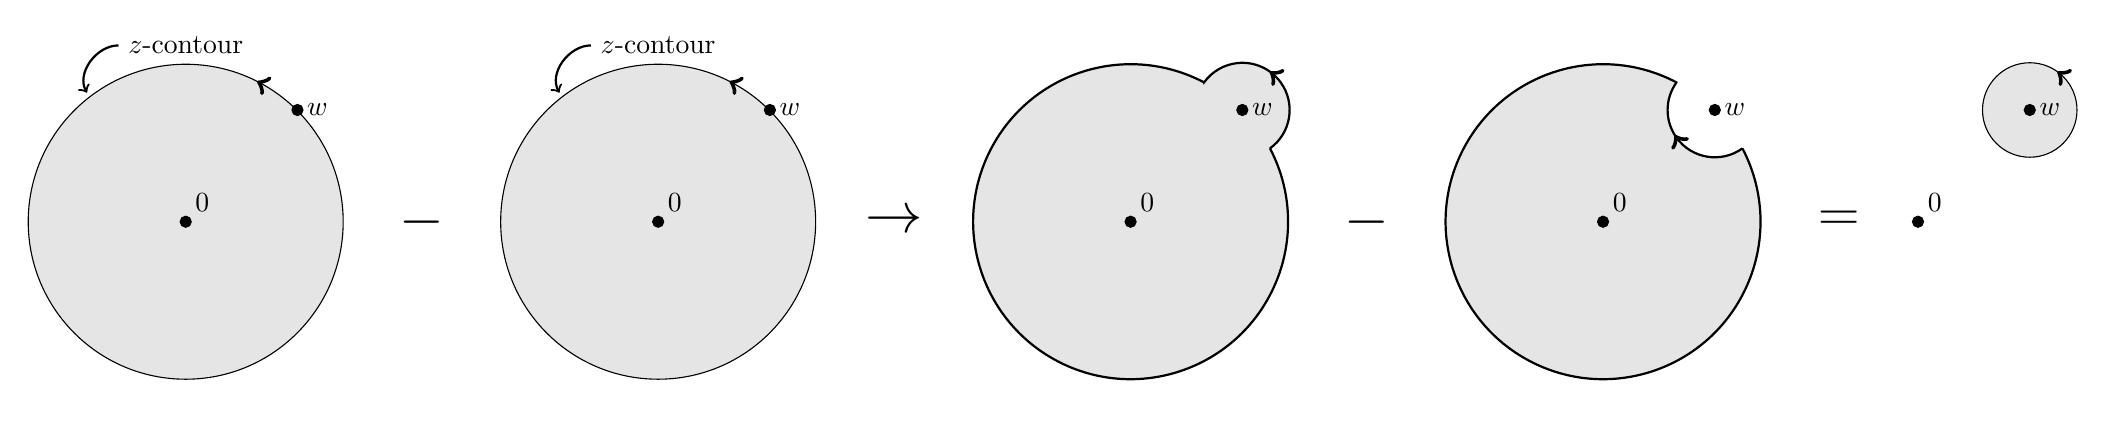
\begin{tikzpicture}

  \node [style={circle,minimum width=4cm,fill=gray!20},draw=black,name path=A,decoration={markings,mark=at position 0.175 with {\arrow[ultra thick]{>}}},postaction={decorate}] at (0,0) (A) {};
  \node [style={circle,minimum width=1.2cm},name path=C] at (A.north east) (B) {};
  \filldraw (A) circle (2pt) node [above right] {0} (B) circle (2pt) node [right]{$w$};
  \node [above] at (A.north) (annotation) {$z$-contour};
  \draw [thick] (annotation.west) edge[out=180,in=120,->] ++(-0.4,-0.6);

  \node [style={circle,minimum width=4cm,fill=gray!20},draw=black,name path=C,decoration={markings,mark=at position 0.175 with {\arrow[ultra thick]{>}}},postaction={decorate}] at (6cm,0) (C) {};
  \node [style={circle,minimum width=1.2cm},name path=D] at (C.north east) (D) {};
  \filldraw (C) circle (2pt) node [above right] {0} (D) circle (2pt) node [right]{$w$};
  \node [above] at (C.north) (annotation) {$z$-contour};
  \draw [thick] (annotation.west) edge[out=180,in=120,->] ++(-0.4,-0.6);

  \node [style={circle,minimum width=4cm,fill=gray!20},name path=E] at (12cm,0) (E) {};
  \node [style={circle,minimum width=1.2cm,fill=gray!20},name path=F,decoration={markings,mark=at position 0.15 with {\arrow[ultra thick]{>}}},postaction={decorate}] at (E.north east) (F) {};
  \filldraw (E) circle (2pt) node [above right] {0} (F) circle (2pt) node [right]{$w$};

  % intersection points between circles E and F
  \path [name intersections={of = E and F}];
  \coordinate (EF1) at (intersection-1);
  \coordinate (EF2) at (intersection-2);

  % calculate angles from center of E/F to intersection points
  \pgfmathanglebetweenpoints{\pgfpointanchor{E}{center}}{\pgfpointanchor{EF1}{center}}
  \let\EEFone\pgfmathresult

  \pgfmathanglebetweenpoints{\pgfpointanchor{E}{center}}{\pgfpointanchor{EF2}{center}}
  \let\EEFtwo\pgfmathresult

  \pgfmathanglebetweenpoints{\pgfpointanchor{F}{center}}{\pgfpointanchor{EF1}{center}}
  \let\FEFone\pgfmathresult

  \pgfmathanglebetweenpoints{\pgfpointanchor{F}{center}}{\pgfpointanchor{EF2}{center}}
  \let\FEFtwo\pgfmathresult

  % draw outline
  \draw[thick]
  (EF2) arc[start angle=\FEFtwo-360, end angle=\FEFone,radius=0.6cm] --
  (EF1) arc[start angle=\EEFone-360, end angle=\EEFtwo,radius=2cm];

  \node [style={circle,minimum width=4cm,fill=gray!20},name path=G] at (18cm,0) (G) {};
  \node [style={circle,minimum width=1.2cm,fill=white},name path=H] at (G.north east) (H) {};
  \filldraw (G) circle (2pt) node [above right] {0} (H) circle (2pt) node [right]{$w$};

  % intersection points between circles G and H
  \path [name intersections={of = G and H}];
  \coordinate (GH1) at (intersection-1);
  \coordinate (GH2) at (intersection-2);

  % draw outline
  \draw[thick,decoration={markings, mark=at position 0.075 with {\arrow[ultra thick]{>}}},postaction={decorate}]
  (GH2) arc[start angle=\FEFtwo-360, end angle=\FEFone-360,radius=0.6cm] --
  (GH1) arc[start angle=\EEFone-360, end angle=\EEFtwo,radius=2cm];

  \node [style={circle,minimum width=4cm}] at (22cm,0) (E) {};
  \node [style={circle,minimum width=1.2cm,draw=black,fill=gray!20},decoration={markings,mark=at position 0.15 with {\arrow[ultra thick]{>}}},postaction={decorate}] at (E.north east) (F) {};
  \filldraw (E) circle (2pt) node [above right] {0} (F) circle (2pt) node [right]{$w$};

  {\huge
  \draw (3cm,0) node {$-$} (9cm,0) node {$\to$} (15cm,0) node {$-$} (21cm,0) node {$=$};
  }

\end{tikzpicture}

\end{document}
